\chapter{Background Study}
\label{chapter:context}
\pagebreak

\textbf{Chapter Abstract}

This chapter introduces the background of this thesis work by giving a general presentation on notions and current state-of-the-art in the domain of Virtual Reality (VR) and Computer Supported Collaborative Work (CSCW), and also by presenting research questions and existing work on how users collaborate in immersive collaborative virtual environments (CVEs).

\vspace*{2\baselineskip}

\minitoc

\newpage
\section{Introduction}
Virtual reality (VR) technology provides users with new interaction possibilities by offering perceptual immersion and real time interaction through sensorimotor interfaces in a virtual space. VR technology has been applied in various domains from industrial product design to training, from education to entertainment. With rapid increasing computation capacity and high-speed computer network, computer-generated virtual environments can be interconnected to achieve group immersion. So both co-located and remote users can be connected to a same virtual environment to accomplish collaborative tasks.
 
This chapter presents the general background of this thesis by discussing different topics related to collaboration in immersive virtual environments. It is divided into three main sections. The first explores key components of virtual reality technology, from its definition to the current state-of-the-art of advances in technical and social aspects. The second presents research around human collaborative work and how they could be supported by modern computer systems. It also shows issues and challenges of collaborative virtual environments (CVEs), which is a virtual environment shared by networked users. The last section addresses how networked immersive experience changes the way users communicate and interact with each other and summarizes existing work from a user-centered perspective.


\section{Virtual Reality}
\subsection{Definition}
Virtual reality related devices appeared before the term itself was created. The \textit{Sensorama Machine} invented in 1957 and patented in 1962 by Morton Heiling believes to be the first multi-sensorial application (Figure~\ref{fig:1_earlyapp}-left). It is a simulator which provides the illusion of reality using a 3-D motion picture with smell, stereo sound, vibrations of the seat, and wind in the hair to create the illusion\footnote{http://www.mortonheilig.com/InventorVR.html}. Then in 1968, Ivan Sutherland with the help of his student Bob Sproull created the first virtual reality and augmented reality (partly see-through) headset named ``The Sword of Damocles" \citep{Sutherland1968Hmd} (Figure~\ref{fig:1_earlyapp}-right).

\begin{figure}[htb]
  \centering
  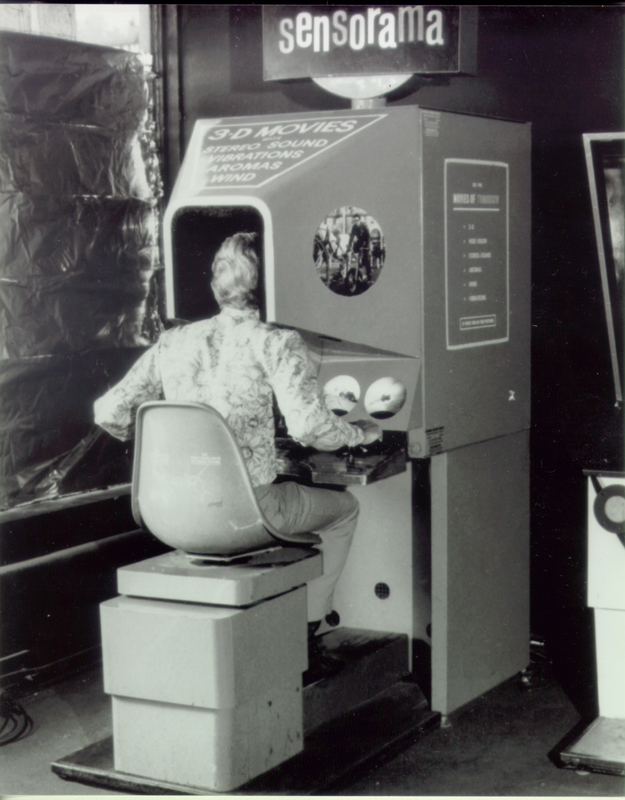
\includegraphics[height=7.5cm]{figures/ch1/sensorama}
  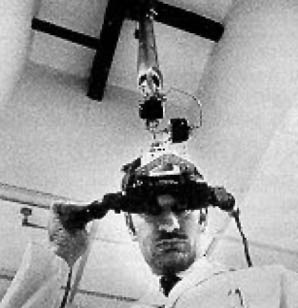
\includegraphics[height=7.5cm]{figures/ch1/ultimateHMD}
  \caption{\label{fig:1_earlyapp}First virtual reality applications: Sensorama Machine (left); The first head mounted display (right).}
\end{figure}

The term ``Virtual reality" in its modern usage was coined and popularized by Jaron Lanier \citep{Lanier1992VR} through his company VPL Research in 1980's. Early definitions of virtual reality are often device-oriented which refer to a certain type of sophisticated computer equipment serving as a medium to connect users to a digitally created space. In the meanwhile, researchers began to discuss and establish conceptual framework of virtual reality, switching from device-oriented definitions to user experience based understanding. Especially, the term ``presence" or ``telepresence" was introduced to describe the generic perception of being in an artificial environment \citep{Sheridan1992MTV}, which is one of the key notions of VR and will be discussed more thoroughly later on. More elaborated discussions about the history and definition of virtual reality can be found in \citet{Rheingold1991VR}'s book and \citet{Steuer1995Defining}'s paper.

Nowadays, a relatively complete definition of virtual reality was given by another book of \citet{Fuchs2011Book}: ``Virtual reality is a scientific and technical domain that uses computer science and behavioral interfaces to simulate in a virtual world the behavior of 3D entities, which interact in real time with each other and with one or more users in pseudo-natural immersion via sensorimotor channels."

This definition covers three important aspects of virtual reality:

First, virtual reality is both a technical and scientific domain. On one hand, technological progress makes unthinkable experiences become available and provides a hardware platform on which theoretical research of virtual reality is based. For example, CAVE and Head-Mounted Display bring a higher level of visual immersion so that users can actually ``step in" the virtual world and have the sensation of ``being at another place". Real-time tracking devices like leap motion and kinect enable motion capture so that users can interact with computers using natural gestures and other types of body movement. On the other hand, researchers make further investigations of the cause and influencing factors of user's subjective feelings using existing devices, and in return, provide guidelines for the development of future virtual reality systems.

Virtual reality is an extension of human computer interaction (HCI) as we move from traditional desktop to 3D user interface, many of its research methods are inherited or inspired by HCI research work. However, unlike HCI which is design-oriented and tries to find efficient, ergonomic and aesthetic interfaces for interaction, virtual reality aims to ``remove" this interface and let users interact naturally with the virtual world. Virtual reality groups research efforts from various domains as it relies on different technical science domains (e.g. computer science, robotics and automatics etc.) and also on contributions from human and behavioral science (e.g. cognitive psychology, physiology, neurobiology, etc.).

Second, virtual reality possesses two key characteristics that distinguish itself with other existing technologies related to 3D virtual environment: sensorial immersion and real time interaction. In desktop or console based video games, players enjoy real time interaction in the virtual world alone or with other players. They use input devices like joystick, mouse and keyboard that offer very limited sensorial immersion. On the contrary, 3D movies projected on large screens in the cinema give the audience good visual immersion, but no interaction capability. The emergence of virtual reality technology brings great changes to the way we are connected to the virtual world. Having the feeling of being immersed in another world and being able to interact in real time in that world as naturally as in the real world is quite appealing and may change completely the game and movie industries. Of course, the application of virtual reality technology is not limited to these domains, it also has great impact on education, product design, training, etc. \citep{Hale2014Handbook}.

Last and the most important, it reveals three main components of virtual reality system: the virtual environment, the user, and the behavioral interface allowing them to interact. The ``perception, decision and action" loop \citep{Fuchs2011Book} describes how users interact with the surrounding virtual world, which is a transposition of the ``perception, cognition, action" loop demonstrating man's behavior in a real world. As shown in Figure~\ref{fig:1_loop}, the user acts (vocal commands, gestures and other body movements, etc.) on the virtual world through motor interfaces, and these activities are captured and transferred to the computer system. Then the computer system makes corresponding changes to the virtual world and generates sensorial reactions (images, sound, haptic, etc.) that are transferred to the user via sensorial interfaces.

\begin{figure}[htb]
  \centering
  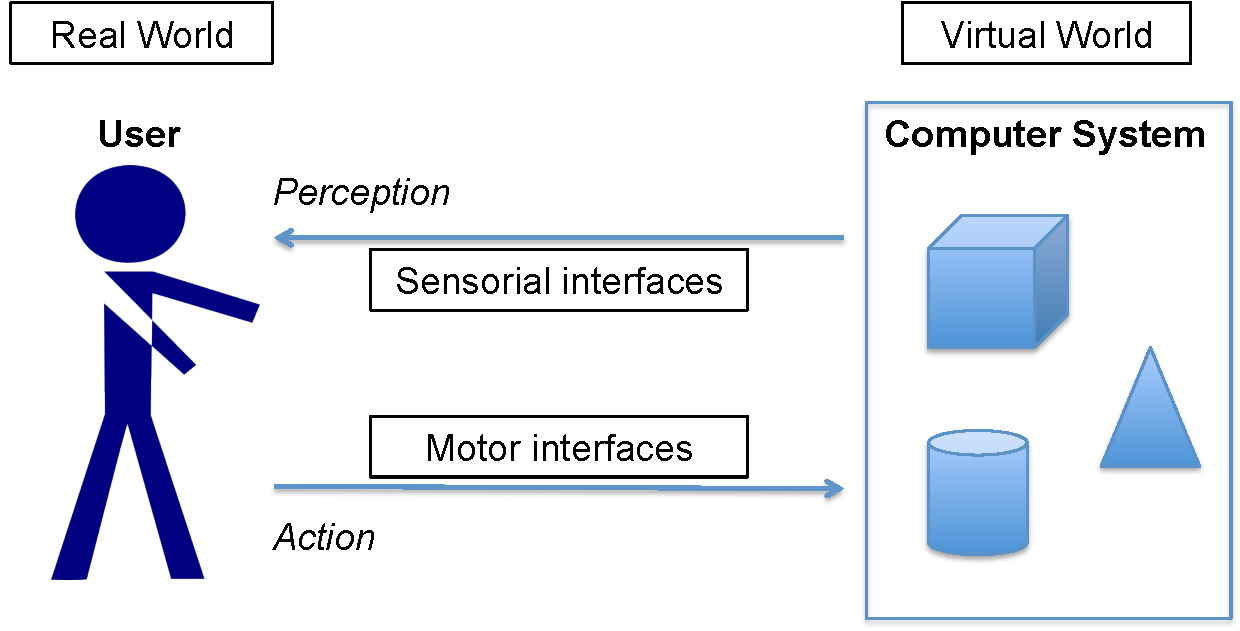
\includegraphics[width=0.9\textwidth]{figures/ch1/loop}
  \caption{\label{fig:1_loop}The ``perception, decision and action" loop in interactive virtual environment.}
\end{figure}

Since the virtual world is totally generated by the computer system, two inherent issues need to be solved: the latency and the sensorimotor discrepancies. The latency is the time lag between the user's action on motor interfaces and the perception of the consequences of this action on the virtual environment through sensorial interfaces. This artifact influences every virtual reality application and may be the source of many problems related to user comfort. The sensorimotor discrepancy is another problem for virtual reality applications. With technical progression, we can simulate more complex phenomena and provide more interaction through sensorimotor interfaces in the virtual environment, but the real world offers way more information for us to simulate with current technology and the sensorimotor discrepancies will continue to exist.

Now we will discuss in more details about the three components of virtual reality system mentioned above: the virtual environment, the behavioral interfaces and the human inside.

\subsection{Virtual Environment}
Virtual environment is a term often used to describe computer-generated synthetic space, similar to virtual world. However, more strictly speaking, as \citet{Ellis1991VE} explained, an environment is the theater of human activity, so virtual environment is a human-centered notion, not only refers to the digital data that forms an artificial world. For example, according to \citet{Fox2009Guide}: ``A virtual environment is a digital space in which a user's movements are tracked and his or her surroundings rendered, or digitally composed and displayed to the senses, in accordance with those movements." This definition emphasizes that a virtual environment is a virtual space that can react to user's movements and change accordingly.

\citet{Ellis1991VE} summarized three parts which form a virtual environment: content, geometry and dynamics. The content is often organized as scene graph with clear hierarchical structure and inter relationship between objects. Each object possesses a state vector containing properties such as position, orientation, velocity and color, etc. The geometry is a description of an environmental field of action that has dimensionality, metrics and extent, and the dynamics of an environment are the rules of interaction among its contents describing their behavior, such as physical laws (gravity, object collision, etc.). More details on the description of virtual environment can be found in \citet{Ellis1991Pictorial}'s book.

In virtual reality applications, the diversity of origins of the worlds represented in the virtual environment makes virtual reality more than a simple copy of the ``reality" that we live in. As summarized by \citet{Fuchs2011Book}, the virtual world could be a simulation of certain aspects of the real world, but also a completely symbolic or imaginary world. The visual representation of objects could vary depending on our need, and spatial, temporal and physical laws may or may not be applied in the virtual world. For example, we can visualize and interact with structure of molecules, flow of fluids under different scales \citep{Ferey2009Multisensory, Bryson1996Virtual}, we can also change the speed of light to better visualize and understand phenomena of relativity \citep{Doat2011NRP}, or the entire world could just be a figment of imagination of an artist or a science-fiction writer.


\subsection{Behavioral Interfaces}
As mentioned in \citet{Fuchs2011Book}'s definition of virtual reality, behavioral interface is a term to describe a type of interfaces that connect the user to the virtual environment. Unlike traditional human computer interfaces which act as a communication tool (e.g. keyboard), behavioral interfaces use the motricity or perceptions of human resulting from his/her behavior in the real world to carry out activities in a virtual world. As shown in Figure~\ref{fig:1_loop}, two types of behavioral interface exist: sensorial interfaces are designed to transfer sensory stimuli from computer to the user while the motor interfaces transfer motor responses from the user to the computer, thus we can also call them sensorimotor interfaces. One of the current challenges of virtual reality is to build more efficient and transparent interfaces based on human sensory channels and motor activities.

\subsubsection{Visual Interface}
\label{sec:visual_interface}
As the idiom ``Seeing is believing" states, the visual sense is nearly the most important sensory channel that humans use to discover the real world, which is also true in virtual reality applications. The software and hardware advancements in computer graphics constantly improve the quality of real time three-dimensional images, which allows more complex and photo-realistic rendering. The display used as visual interface should have the following characteristics:

\begin{itemize}
\item Large field of view (FoV) (``borderless");
\item Stereoscopic vision in the entire binocular field of vision;
\item High graphic resolution (pixel density), currently most widely used is 1080p FullHD display, but displays with higher resolution are on the way;
\item Head (even eye) tracking compatible. Since we can move our head and eyes to look into different directions, it is necessary to assure that user always has perspective-correct view of the virtual scene. This can be achieved by using tracking devices\footnote{see section \ref{sec:tracking}.}
\end{itemize}

A lot of display systems exist nowadays which satisfy all or part of the characteristics listed above, from large immersive rooms and wall displays to table-sized screen, and even portable screens mounted on user's head (see Figure~\ref{fig:1_vi}). They vary in size, form, display technology and aimed applications. Only CAVE (Figure~\ref{fig:1_vi:cave}) and HMD (Figure~\ref{fig:1_vi:hmd}) are designed to provide fully visual immersion. Other displays, on the contrary, can not assure a user to always stay visually inside the virtual world, but they can offer good visual immersion and are better suited for data visualization and 3D object interaction in certain cases. There are also some special display solutions not mentioned above that can provide individual stereoscopic views of 3D models such as the volumetric display \citep{Grossman2008Volum} and holographic display \citep{Lucente1997Holo}, but currently they can only be applied to non-immersive context with contents that are difficult to be changed in real time.


\begin{figure}[htb]
  \begin{subfigure}{.3\textwidth}
    \centering
    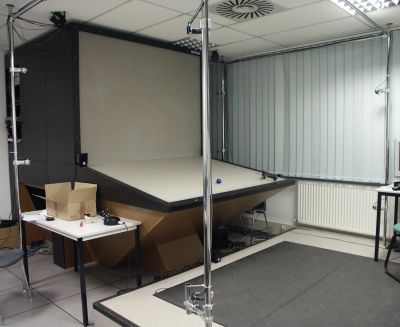
\includegraphics[height=3.5cm]{figures/ch1/workbench}
    \caption{Workbench formed by two separate screens (LIRIS-CNRS).}
    \label{fig:1_vi:bench}
  \end{subfigure}
  \begin{subfigure}{.3\textwidth}
    \centering
    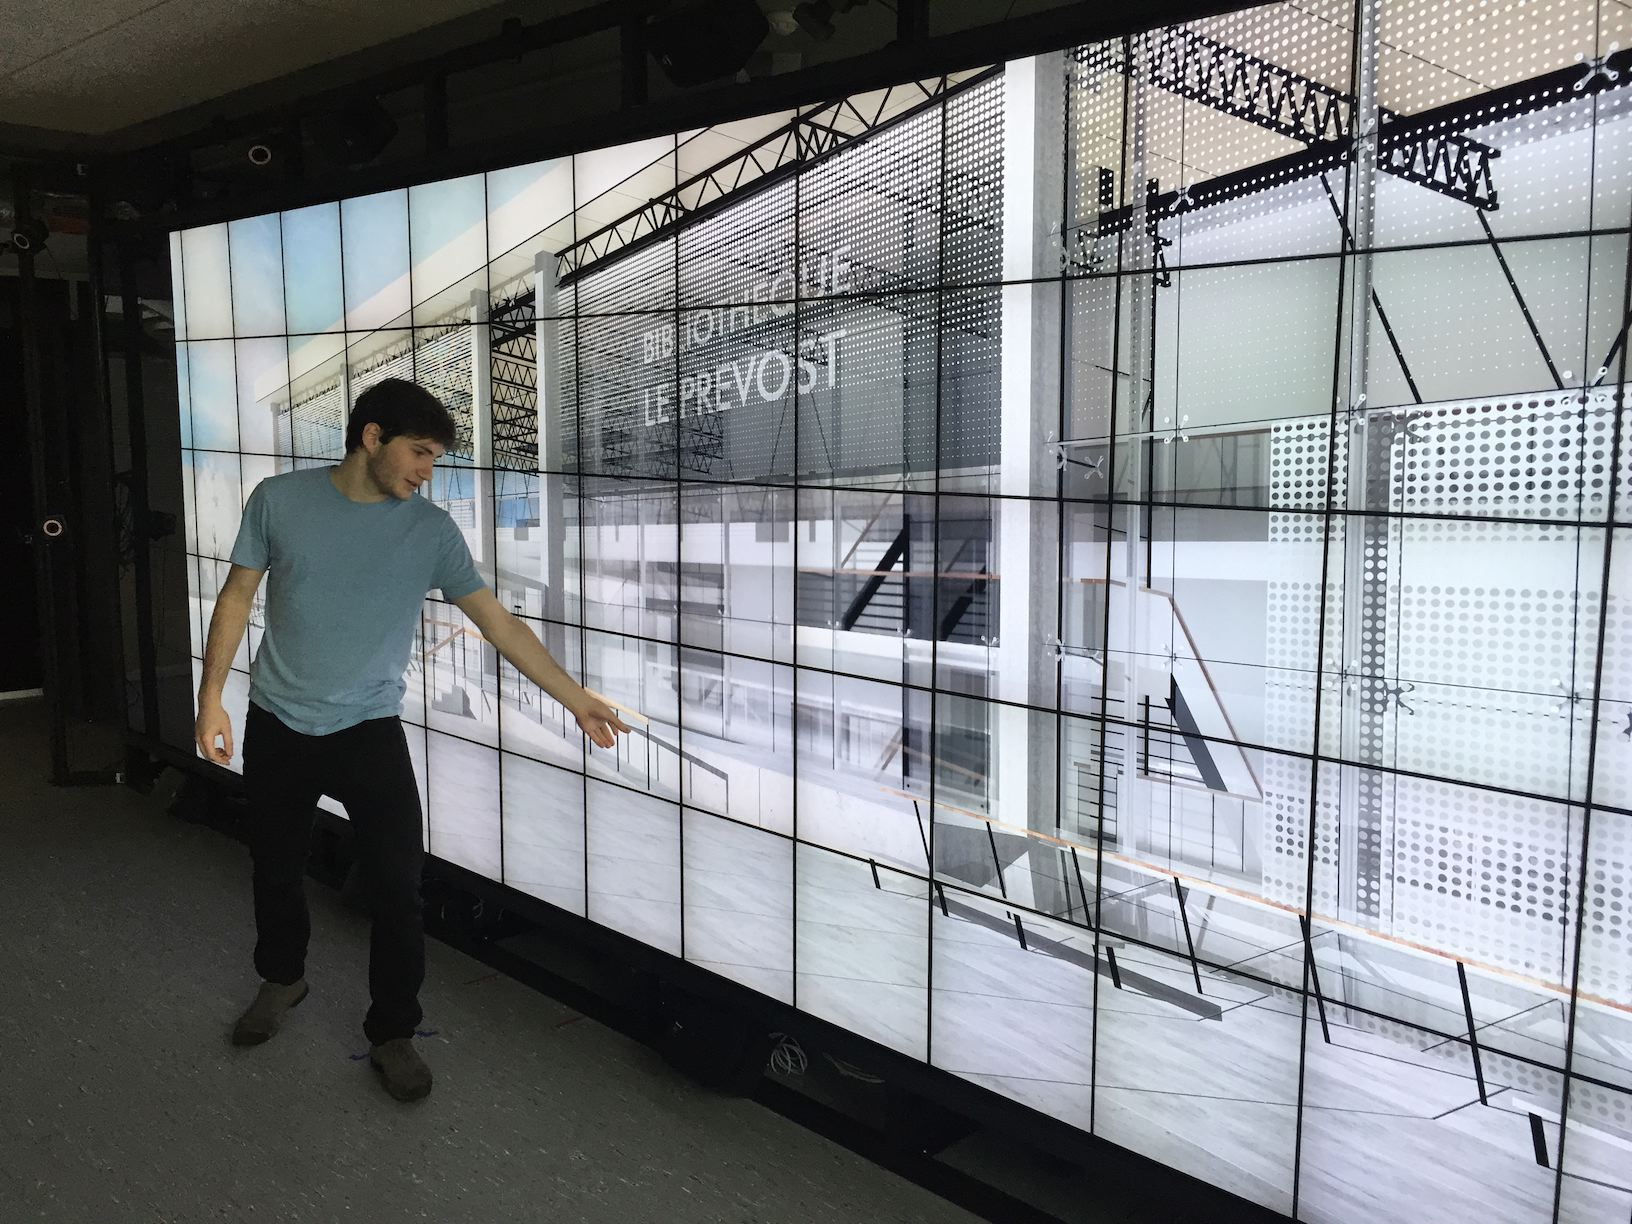
\includegraphics[height=3.3cm]{figures/ch1/wilder}
    \caption{Large image wall composed of high resolution touch screens (WILDER, in$\lvert$situ$\rvert$, LRI).}
    \label{fig:1_vi:wall}
  \end{subfigure}
  \begin{subfigure}{.3\textwidth}
    \centering
    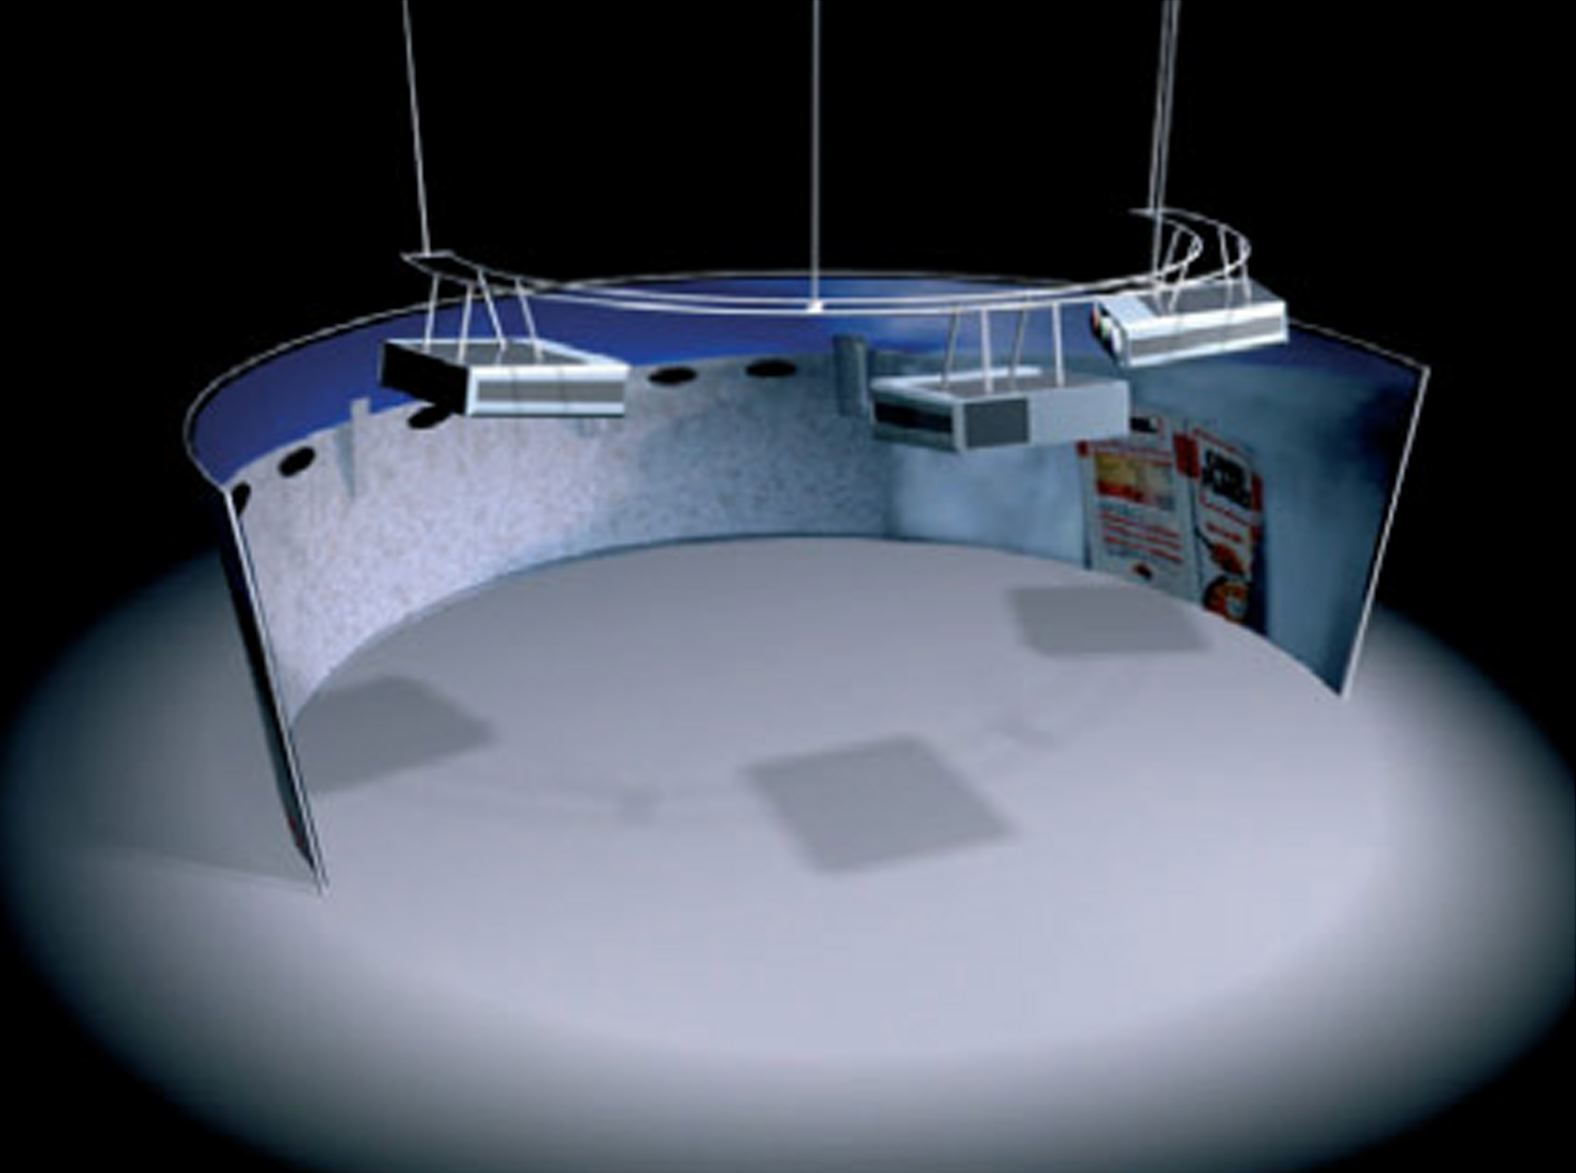
\includegraphics[height=3.5cm]{figures/ch1/icone}
    \caption{The curved panoramic projection screen i-Cone\texttrademark{} \citep{Simon2002Icone}.}
    \label{fig:1_vi:icone}
  \end{subfigure}
  \begin{subfigure}{.5\textwidth}
    \centering
    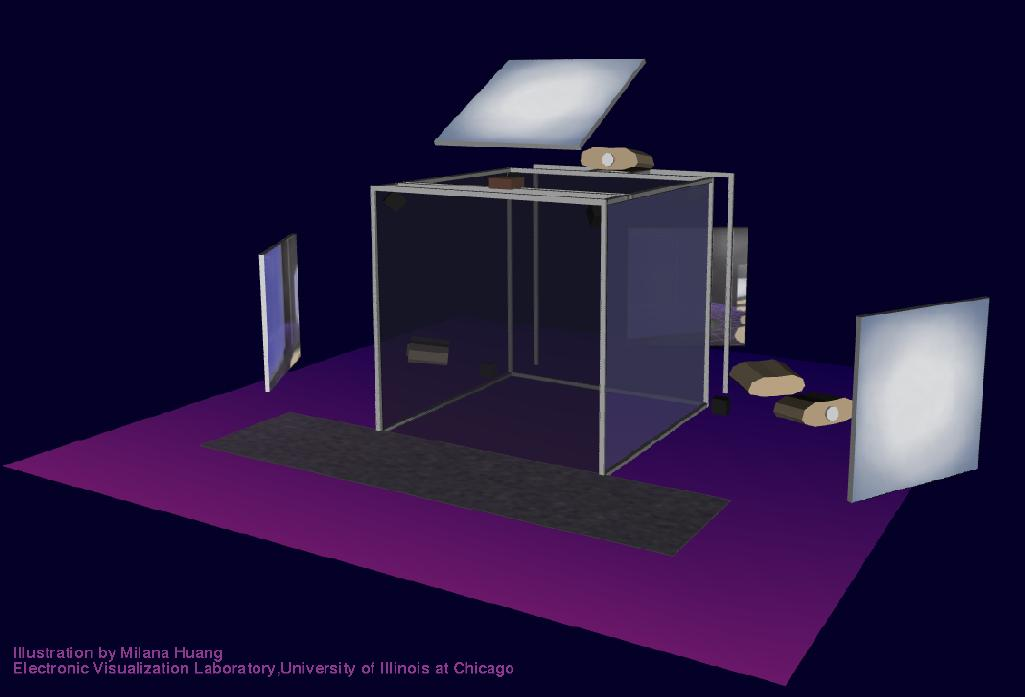
\includegraphics[width=0.9\linewidth]{figures/ch1/cave}
    \caption{CAVE\texttrademark{}: Cave Automatic Virtual Environment \citep{CruzNeira1992CAV}.}
    \label{fig:1_vi:cave}
  \end{subfigure}
  \begin{subfigure}{.45\textwidth}
    \centering
    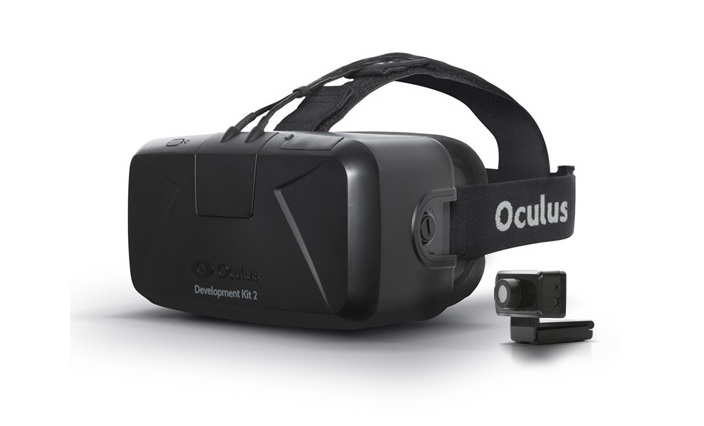
\includegraphics[width=\linewidth]{figures/ch1/oculus}
    \caption{Head-Mounted Display (HMD): Oculus DK2 \copyright{} Oculus VR LLC.}
    \label{fig:1_vi:hmd}
  \end{subfigure}
  
  \caption{\label{fig:1_vi}Different types of visual interfaces.}
\end{figure}


\subsubsection{Audio Interface}
Audio cues are very important for us to perceive events happen in the real world, similarly, the virtual world would be much less appealing if there is no sound. A virtual object would be more ``realistic" if there is a corresponding spatialized sound combined with its visual representation displayed in stereoscopy. For example, a virtual telephone displayed in front of a user with a ringtone coming exactly from that location would make the user believe that the telephone is ringing. 3D audio sometimes has more contributions to the immersion level because it allows users to perceive objects behind them and also objects that are beyond their vision scope. A virtual environment filled with ambiance noises and spatialized sound coming from different virtual entities can enhance user's feeling of ``being in that world".

Audio interface has two types of roles: (1) to capture and transfer the sound made by the user (speech, hand clapping, etc.) to the computer system; (2) to transfer audio stimuli from the virtual environment (and from other users connected to the same VE) to the user. The implementation of binaural audio interface managing spatialized sound requires quite complex hardware and software setup which involves lots of research and engineering efforts \citep{Begault1994Sound}.

Currently three solutions exist: first, ambisonic sound can be reproduced by a group of loudspeakers situated around the user. This kind of setup can be used to simulate ambient noises or audio sources coming from places farther than the perimeter of the loudspeaker group; second, based on Head-Related Transfer Function (HRTF) \citep{Kistler1992HRTF} which is a response that characterizes how an ear receives a sound from a point in space, binaural sound can be reproduced for multiple users by equipping each of them a stereo headphone combined with head tracking; at last, we can use a matrix of micro loudspeakers to reproduce physically the acoustic field based on Wave Field Synthesis \citep{Verheijen1998WFS}, which is independent with listener's position. The headphone-based binaural sound is a more portable and lightweight solution while the other two methods require more complex hardware setup and are more suitable for large acoustic rooms or theaters. Moreover, the Wave Field Synthesis method can not be combined with retro-projection based immersive display as the loudspeaker matrix behind the screen would occlude projected images.

\subsubsection{Tracking Interface}
\label{sec:tracking}
The goal of tracking interface is to capture and transfer user's motor information as input for the computer system to update the virtual world and to generate proper sensorial stimuli (visual, audio, etc.) for the user. Tracking an entity in 3D space requires six degrees of freedom (DoF) information: three for position in form of a vector $(x, y, z)$ and three for orientation in form of Euler angle $(\theta{x},\theta{y},\theta{z})$.

In many virtual reality applications, it is sufficient to track user's head and dominant hand to respectively ensure correct visual rendering according to user's viewpoint and to allow basic interaction (e.g. object selection) in the virtual world. However, full-body movement tracking (motion capture) is increasingly demanded to enrich interaction scenarios and to enhance the level of immersion. Moreover, when multiple users are inside the same virtual environment, full-body tracking combined with decent avatar representations largely facilitate social human communication (which will be further discussed in section~\ref{sec:user-com}) by transferring subtle non-verbal cues (postures and gestures) among users. Recently, eye tracking technology has received a lot of attentions for its potential benefits in many domains \citep{Duchowski2007Eye} and it will become an important part of tracking interface for virtual reality systems.

Tracking interface can be implemented with different physical principals, including mechanical, electromagnetic, optical or acoustic methods \citep{Meyer1992Survey}. Although no single technology works for all purposes, certain methods work quite well for specific applications \citep{Welch2002Survey}. The new trend now is to combine different tracking technologies into one product to get better tracking quality, e.g. the hybrid suit from ART\footnote{http://www.ar-tracking.com/products/motion-capture/hybrid-suit} is a combination of optical, mechanical and magnetic trackers. Video based tracking devices using computer vision methods, such as kinect and leap motion (Figure~\ref{fig:1_video_tracking}), are also getting more popular because of their low cost and easy setup procedure.

\begin{figure}[htb]
  \begin{subfigure}{.5\textwidth}
    \centering
    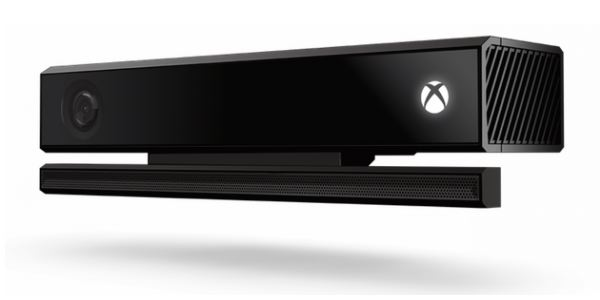
\includegraphics[height=3cm]{figures/ch1/kinect}
    \caption{The Kinect (version 2) \copyright{} Microsoft.}
    \label{fig:1_video_tracking:kinect}
  \end{subfigure}
  \begin{subfigure}{.5\textwidth}
    \centering
    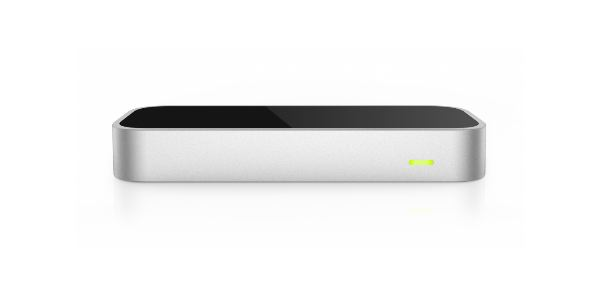
\includegraphics[height=3cm]{figures/ch1/leap}
    \caption{Leap motion controller \copyright{} Leap Motion.}
    \label{fig:1_video_tracking:leap}
  \end{subfigure}
  \caption{\label{fig:1_video_tracking}Video-based tracking interfaces.}
\end{figure}

\subsubsection{Haptic Interface}
The word \textit{haptic} coming from Greek means ``pertaining to the sense of touch". Haptic technology was first developed for tele-operation task so that users can enhance the remote control of machines and devices. Now more and more virtual reality applications integrate haptic interface so users can ``tele-operate" objects in the virtual world. With the help of haptic feedback, users can not only perceive virtual objects' different properties (shape and texture, etc.) by touch, but also interact physically with them (e.g. to push a virtual forklift \citep{Martin2012Forklift}). Being able to imply the sense of touch in the interaction within virtual environment is a huge step forward in aim of creating fully immersive experience in the virtual world, though lots of technical issues remain to be solved. 

Generally speaking, haptic technology aims to recreate the sense of touch by applying two kinds of stimuli to the user: tactile feedback and proprioception feedback. Tactile sensation is formed from several modalities including pressure, skin stretch, vibration and temperature, while proprioception feedback concerns the feeling of having physical contact between different parts of human body and the virtual environment. Many haptic devices on the market provide force feedback and vibration for part of the human body, especially the hands and arms, for example, electromechanical haptic arms shown from Figure~\ref{fig:1_hi:phantom} to \ref{fig:1_hi:scale1} have different workspace size and accessible force range to provide from desktop-based to room-sized haptic interaction. Some glove-shaped (Figure~\ref{fig:1_hi:dexmo}) or string-based (Figure~\ref{fig:1_hi:spidar}) devices equipped with finger-level motors can support even finer force feedback to the user for actions like object grasping and manipulating with fingers. However, there seems still no easy solution to provide full-body haptic feedback and tactile experience with relatively complex objects, so sometimes real objects (called props or tangible interfaces) are introduced into the virtual environment for passive haptic feedback in specific applications (Figure~\ref{fig:1_hi:prop}).

\begin{figure}[htb]
  \begin{subfigure}{.3\textwidth}
    \centering
    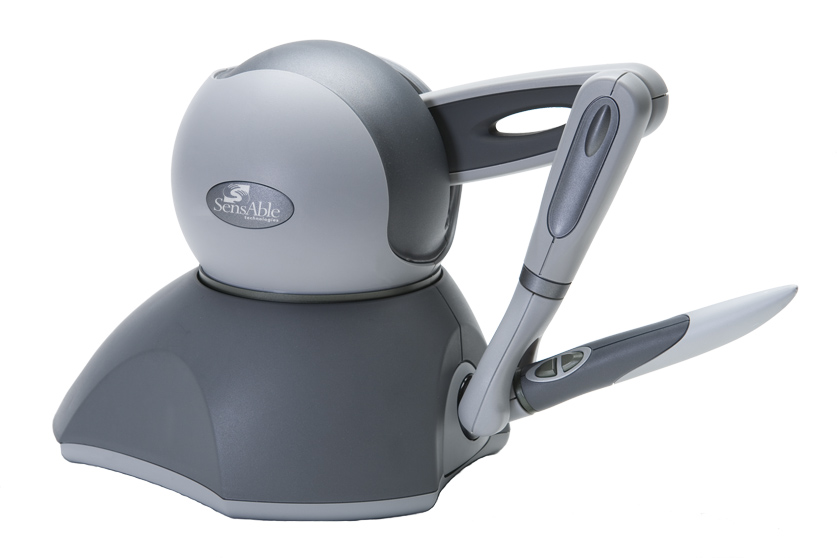
\includegraphics[width=0.8\linewidth]{figures/ch1/phantom}
    \caption{PHANTOM\textregistered{} Omni haptic arm \copyright{} Sensable.}
    \label{fig:1_hi:phantom}
  \end{subfigure}
  \begin{subfigure}{.3\textwidth}
    \centering
    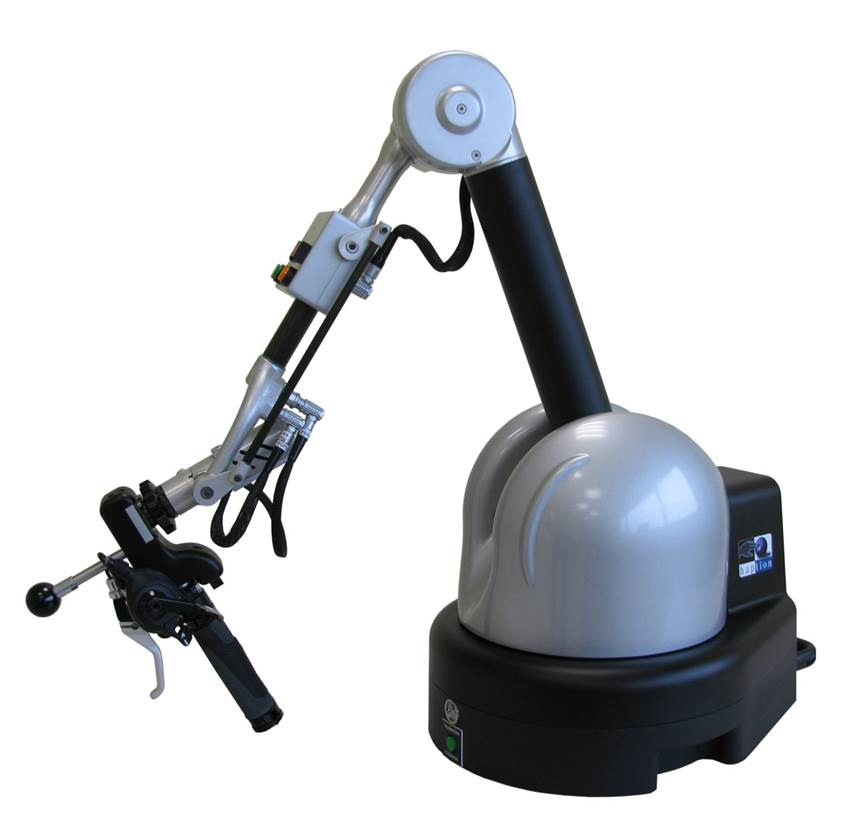
\includegraphics[width=0.8\linewidth]{figures/ch1/virtuose}
    \caption{The Virtuose 6D haptic arm \copyright{} Haption.}
    \label{fig:1_hi:virtuose}
  \end{subfigure}
  \begin{subfigure}{.35\textwidth}
    \centering
    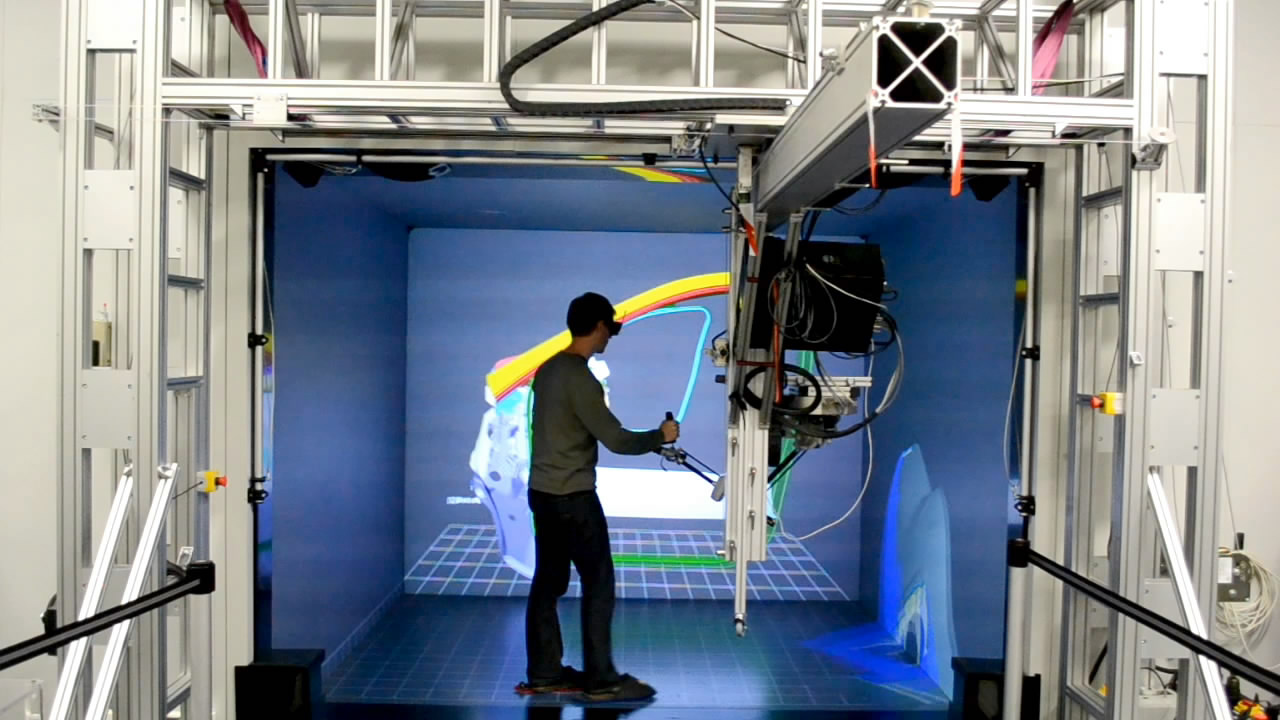
\includegraphics[width=0.9\linewidth]{figures/ch1/scale1}
    \caption{Scale 1\texttrademark{} room-sized haptic solution \copyright{} Haption.}
    \label{fig:1_hi:scale1}
  \end{subfigure}
  \begin{subfigure}{.3\textwidth}
    \centering
    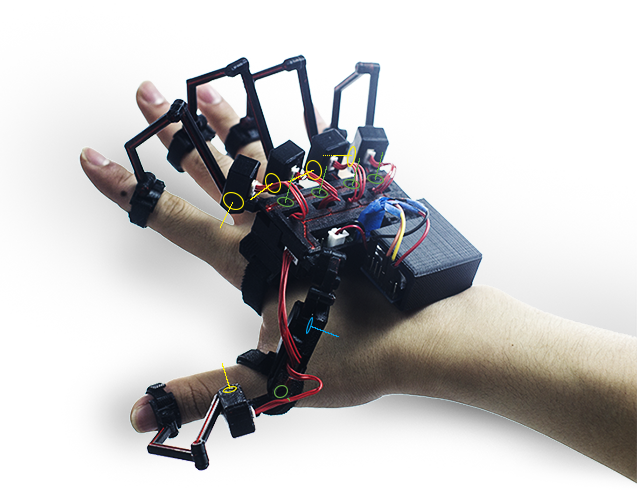
\includegraphics[width=\linewidth]{figures/ch1/dexmo}
    \caption{Dexmo\textregistered{} wearable mechanical exoskeleton \copyright{} Dexta Robotics.}
    \label{fig:1_hi:dexmo}
  \end{subfigure} 
  \begin{subfigure}{.35\textwidth}
    \centering
    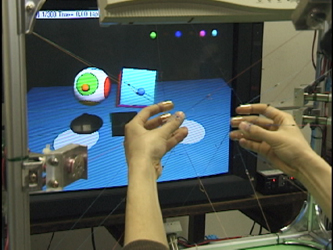
\includegraphics[width=0.9\linewidth]{figures/ch1/spidar}
    \caption{SPIDAR: string-based force feedback device \citep{Sato2002SPIDAR}.}
    \label{fig:1_hi:spidar}
  \end{subfigure}
  \begin{subfigure}{.32\textwidth}
    \centering
    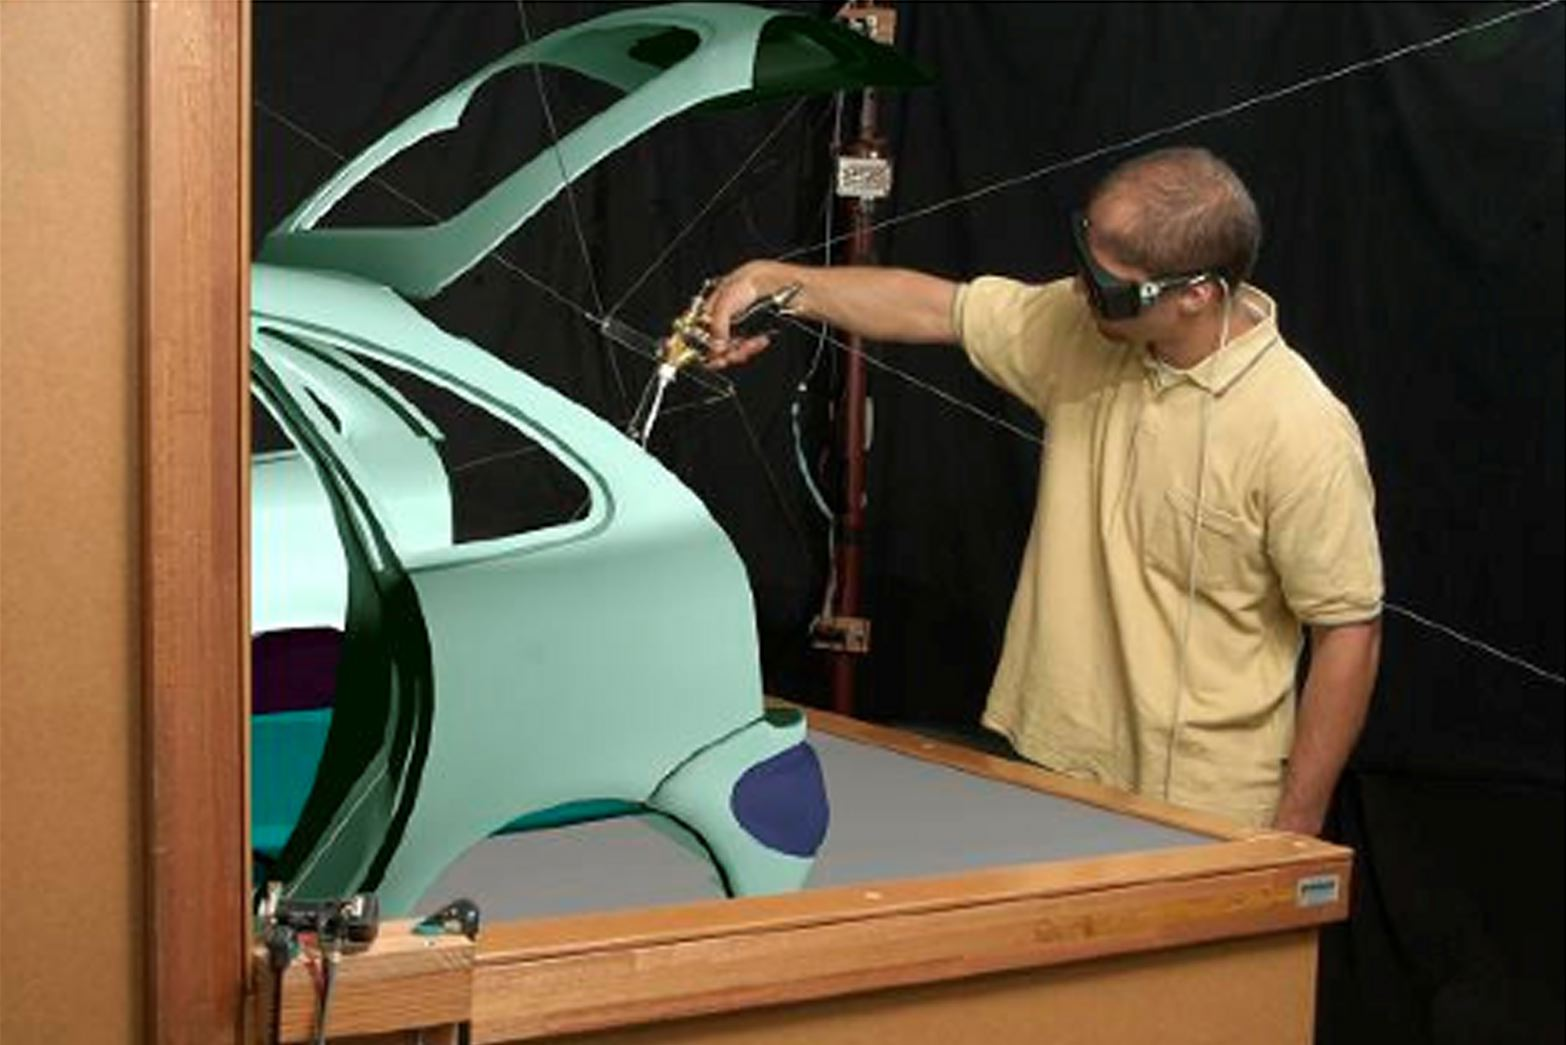
\includegraphics[width=0.9\linewidth]{figures/ch1/prop}
    \caption{The putty gun served as prop offering passive haptic feedback \citep{Ortega2005Prop}.}
    \label{fig:1_hi:prop}
  \end{subfigure}
  \caption{\label{fig:1_hi}Different types of haptic interfaces.}
\end{figure}

\subsubsection{Other Interfaces}
Apart from major sensory channels like vision, audio and the sense of touch, the human sensorimotor system is way more complex and all senses could contribute to the feeling of presence in the virtual world. For example, \citet{Matsukura2011MSF} designed a multi-sensorial field (MSF) display which can generate air flow and odor vapors to simulate odor distribution in the virtual world, and \citet{Narumi2011Flavors} developed a ``Pseudo-gustation" method to change the perceived taste of food by changing its appearance and scent. However, integrating all types of behavioral interfaces into a single virtual environment remains a challenge because of the complexity and compatibility issues of different hardware and software solutions. 


\subsection{Human in Virtual Environment}
As we discussed before, virtual reality is a human-centered research domain. Technical advancement concerning the modeling of virtual world and the design of behavioral interfaces all serve to provide a better feeling of ``being in another world" (presence) for the human in virtual environment. So to understand human activity and sensation at perceptual and cognitive levels is a key to the success of virtual reality system.

\subsubsection{3D Interaction}
\label{sec:3D_inter}
The interaction between the user and 3D virtual world begins once he/she is inside the virtual environment, and these human activities can be divided into some basic behaviors named Virtual Behavioral Primitives (VBP) \citet{Fuchs2011Book}. VBPs can be grouped into five categories:

\begin{itemize}
  \item observation;
  \item moving;
  \item acting;
  \item communicating with others;
  \item application control.
\end{itemize}

In the list above, except for application control, these activities are very similar to what people practice in the real world. Observation is our first triggered action after we dived into a virtual environment, which is a relatively passive action. The only interaction part is that when user turns head or has ocular movements (captured with eye tracking), the system will adapt the visual and audio rendering accordingly. Moving or navigation in the virtual world is also a basic interaction for the user to accomplish various tasks like object searching or transporting, way finding, sightseeing, etc. Besides natural walking, many virtual navigation metaphors are developed to effectuate more efficient virtual viewpoint control under different specific conditions (more details to be presented in Chapter \ref{chapter:colocated_colab}). Regarding ``acting", which is a vague notion, is further broke into object selection, manipulation and symbolic input by \citet{Bowman2004UIT}. The way we interact with virtual object is still quite different than with real objects due to technical limitations (e.g. lack of detailed and robust haptic feedback), thus many interaction metaphors are proposed to enable other forms of interaction \citep{Hand1997Survey}.


\subsubsection{Presence}
Sensorial immersion offered by immersive virtual environment (IVE) can give user the illusion of ``being there" or the feeling of presence \citep{Heeter1992Presence}, which is a central concept of virtual reality. Presence, or telepresence, is used to describe user's subjective feeling of being immersed in a virtual environment, while the term ``immersion" is a product of technology that facilitates the production of multimodal sensory stimuli to the user \citep{Slater1994DepthPre, Bystrom1999Model}. Presence in virtual reality is a psychological state relying on sensorimotor illusion, which is different than the presence feeling at cognitive level that we have in dreams or by reading a book.

Many researchers share this general definition of presence, but there are still nuances in the explanations and interpretations of the definition.

\citet{Slater1994DepthPre} suggest that presence is assessed by the subjects as their sense of ``being there", the extent to which they experienced the virtual environments as more the presenting reality than the real world in which the experiment was taking place, and the extent to which the subject experienced the virtual environments as places visited rather than images seen. Then \citet{Kim1997Telepresence} describe presence as the product of two factors: (1) ``the arrival" or the feeling of being ``there" in the virtual environment, and (2) ``the departure" or the feeling of not being there ``there" in the physical environment. ``The arrival" (or one's involvement in a virtual environment) occurs when an individual concentrates their energy and their attention onto a stimulus and the events happening in the virtual environment, thus permitting the augmentation of the degree of involvement or of presence. Similarly, \citet{Witmer1998MPV} relate presence in part to the concept of attention: presence may vary across a range of values that depends in part on the allocation of attentional resources. They think that both involvement and immersion are necessary for experiencing presence. \citet{Lombard1997Heart} have attempted to offer another explanation of the concept of presence as they define presence as the perceptual illusion of non-mediation, which focuses on the transparency of behavioral interfaces.

Studies have shown that the level of presence has not only a pronounced effect on user's task performance \citep{Dangelo2008Benefits}, but also an impact on the social relationship between collaborators \citep{Slater2000Small}. To step further towards a more complete virtual reality system that could invoke higher level of presence for the user, it is important to identify factors that contribute to the formation of presence and to establish related evaluation models. Being an ongoing research topic, existing models for presence measurement are restricted to subjective rating through questionnaires \citep{Usoh2000Using, Witmer1998MPV}. The use of physiological measures for presence evaluation has been attempted \citep{Meehan2002Physiological}, but we still need more follow-up studies to design a complete evaluation model based on physiological indicators. A detailed analysis of influencing factors of presence and a taxonomy for presence measurement methods are presented by \citet{Schuemie2001Pres}.


\subsubsection{Cybersickness}
Cybersickness is a polygenic \citep{Kennedy1992Simulator} and troublesome problem with current virtual reality technology. Cybersickness, or simulator sickness (they may be different according to \citet{Stanney1997Cybersickness}), is the tendency for some users to exhibit symptoms that parallel symptoms of classical motion sickness both during and after being immersed in virtual environments. Short-term symptoms of cybersickness have been identified after repeated studies \citep{Lawson2002Signs}, but currently we still know little about its long-term effects. It is essential to understand the causes for cybersickness and to find ways to eliminate it for better use of virtual reality technology.

Researchers have tried to identify factors that are susceptible to cause cybersickness when using a virtual environment. For example, \citet{Rich1996AICS} examined the relationship between sensory compatibility and cybersickness symptoms, while \citet{So2002Scene} emphasized that the visual complexity of the virtual scene should also be taken into consideration. \citet{Stanney2002HPIVE} gives us a better global view that addresses different perceptive factors that are susceptible to cause cybersickness. Technical issues such as lags \citep{Pausch1992Literature}, flickers \citep{Harwood1987Temporal}, and individual factors like gender \citep{Biocca1992Will} and age \citep{Reason1975Motion}, all have some influences on the severity of cybersickness symptoms. A more complete list of primary factors that contribute to the cause of cybersickness was provided by \citet{LaViola2000DCV}. He also gave an interesting discussion on three conflicting theories that try to explain the occurrence of cybersickness.

Currently, to evaluate the severity of cybersickness, the Simulator Sickness Questionnaire (SSQ) \citep{Kennedy1993SSQ} remains the reference tool. SSQ groups all symptoms around three main factors: nausea (nausea, stomach awareness, etc.), oculomotor (eyestrain, blurred vision, etc.) and disorientation (dizziness, vertigo). The development of various physiological measurements also begins to show interesting correlation between cybersickness symptoms and various physiological indicators \citep{Kim2005Characteristic, Min2004Psycho, Sugita2008Quantitative}. However, further research efforts are required to establish a valid cybersickness evaluation model based on physiological indicators. The study of physiological responses of human body when exposed to virtual environment will also help us to better understand the cause of cybersickness.

\subsubsection{Workspace Management}
When interacting in an immersive virtual environment, user's sensory channels are partly blocked by the computer system. However, this does not change the fact that the user is still in the real world, thus he/she is constrained by limits of the physical workspace, for example, the user can not cross real walls or screen displays. The implication of these real world constrains on the use of immersive virtual environment is a major issue of this manuscript and will be discussed in Chapter \ref{chapter:colocated_colab}).


\subsection{Summary}
This first part of Chapter \ref{chapter:context} gives a brief introduction of virtual reality around its three main components: virtual environment, behavioral interface and the user. Key notions like presence and cybersickness, as well as different hardware implementations of virtual reality system are presented, so they can be used directly later on in this manuscript. 

% -------------------------------------------------------------------------------------------------

\section{Computer Supported Collaboration}
The development of communicational technology changes the way people work together, for example, telephone and telegraph made the exchange of information much faster than paper-based media. Later on, with the boom of the Internet, emails, forums, video conferences create a tighter link among remote collaborators. However, networked collaboration still faces a lot of difficulties in terms of communication and coordination. For example, how a group of coders can contribute to the same project remains a non-trivial job despite using versioning tools like SVN\footnote{http://subversion.apache.org} or Git\footnote{https://git-scm.com}.

In 1984, Irene Greif of MIT and Paul M. Cashman of Digital Equipment Corporation organized a workshop attended by people from various domains interested in using technology to support people in their work. In this workshop the term Computer Supported Cooperative Work (CSCW) was first mentioned \citep{Grudin1994Computer}, then it becomes a research domain attracting world-wide interests. CSCW studies how computer systems could enable a group of people connected by network to work together efficiently, or as stated by \citet{Carstensen1999CSCW}: ``how collaborative activities and their coordination can be supported by means of computer systems". More details about the history, state-of-the-art and research issues of CSCW can be found in the book of \citet{Beaudouin1999CSCW}.


\subsection{Characteristics of Collaborative Work}
We can learn many things from observation of people working and collaborating in the real world to get some insights into the nature of collaborative work \citep{Churchill1998CVE}. Here are some general points to summarize characteristics of collaborative work:

\paragraph{Collaboration is human-centered} The number and profile of people involved in the task define the general organization for collaboration. For example, small groups are likely to work together in real time with more flexible schedules, communicate informally and share information with minimal cost, while large groups need much more efforts for coordination and more adapted communication technology. The profile of collaborators also matters, if one person is way more experienced than others, it is better to have a leader-follower mode so everyone works around this leader. However, if working capacity is homogeneously distributed and especially, each one has his/her own expertise, it is better to work with equal responsibility for the task.

\paragraph{Collaboration is task-oriented} The nature of the task defines the spatial and temporal constrains for collaboration, or we can say that sometimes people need to collaborate because of some spatial or temporal issues and the task can not be done without combining efforts from different actors. For example, tasks like painting a wall or repairing a car together require people to be co-located, other tasks like operating a TV live show, or having a video conference need synchronous actions. Moreover, complex tasks often consist of different components with inherent logical links and the task can only be accomplished with a certain procedure.

In some collaborative tasks people play similar roles, e.g., two workers try to move a heavy object (\textit{piano movers' problem}), two pilots control the landing of a plane, etc. Whilst in other tasks collaborators can also have distinct roles with different associated competence \citep{Pouliquen2014Role}, e.g. the relationship between trainer and trainee, field operator and online assistant, etc.

\paragraph{Awareness is the base of coordination} Awareness is one's knowledge of task related activities, especially activities of others. As stated by \citet{Dourish1992Awareness}, awareness is an ``understanding of the activities of others, which provides a context for your own activity". This ``context" allows an individual to evaluate his/her actions with respect to group goals and work progress. In addition, awareness may also refer to the knowledge of the state of a task related object (e.g. the history and current state of the shared document for group editing task) and the working atmosphere (whether there is an emergency, whether people are under pressure, etc.).


\paragraph{A shared context is essential} A shared context allows group members to ``stay on the same page" (shared understanding), which largely facilitates their communication and coordination. We can call it a \textit{common ground} \citep{Clark1991Grounding} or \textit{team situation awareness} \citep{Salas1995SA} which is based on the situation awareness of each individual. In conventional situations, a shared context is naturally established by a shared physical and social space. For example, two workers are in the same room, there will not be confusion when one points to a table and says ``Let's move it to the corner". When people are distributed and connected by computer network, it is essential for a successful collaborative system to maintain a shared context by sharing artifacts and activities.

\paragraph{Multiple viewpoints are helpful} A complex task should have multiple representations, each offering a different point of view of the problem or focusing on a specific subtask. In certain cases, one individual may require multiple representations to reflect different aspects of their task, whilst in other cases people with different profiles and skills may require tailored representations to provide information specific to their tasks. Taking an example from \citet{Churchill1998CVE}, people taking part in the architectural design review of a building might only want to see features relating to their specialty in detail. So an electrician might only want to see detailed wiring plans, but not necessarily the plans for the plumbing, except in cases where there was a potential conflict. There are more reasons to vary the representation of a task in a broader social context, for example, companies involved in a same project often need to keep their sensitive data or workflow from others. So when designing computer supported collaborative system, ``WYSIWIS" (What You See Is What I See) \citep{Stefik1987WYSIWIS} may not be a proper choice in many cases.

\paragraph{Transition between shared and individual activities is required} Collaborative scenarios usually contain different coupling stages \citep{Gutwin1998Design, Lissermann2014PMC}: \textit{closely-coupled stage} to solve problems in group and \textit{loosely-coupled stage} to tackle individual subtask. So collaborative work involves the interleaving of individual and group effort, which requires explicit communication and coordination between collaborators. For example, in a car assembly task, workers may need to go to storehouses and fetch a certain component for change from time to time, and then come back to the assembly work. This task contains both individual object-searching and closely coupled interactions for the assembly work. \citet{Isenberg2012Co} further identified a series of eight different collaboration styles and activities that participants adopted during a working session around an interactive table. So a collaborative system should manage group workspace as well as personal workspace, and allow active transition between shared and individual activities.

These characteristics help us to understand the process of collaborative work and offer a guideline for the design of computer supported collaborative system. \citet{Okada2007Collab} proposed a multi-layered hierarchical framework which shows a clear picture of different elements contributing to the collaboration and a structural link between aforementioned characteristics. As shown by Figure~\ref{fig:1_collab_model}, the model consists of four layers and each layer is based on the layer below: spatial and temporal coexistence enables awareness of others' activities, which then allows the exchange of views and opinions, the sharing of knowledge and information, and the distribution of work and operations. At the highest level, the sharing of activities enables the final collaboration between multiple actors with the balance between assertions and cooperations (negotiation).

\begin{figure}[htb]
  \centering
  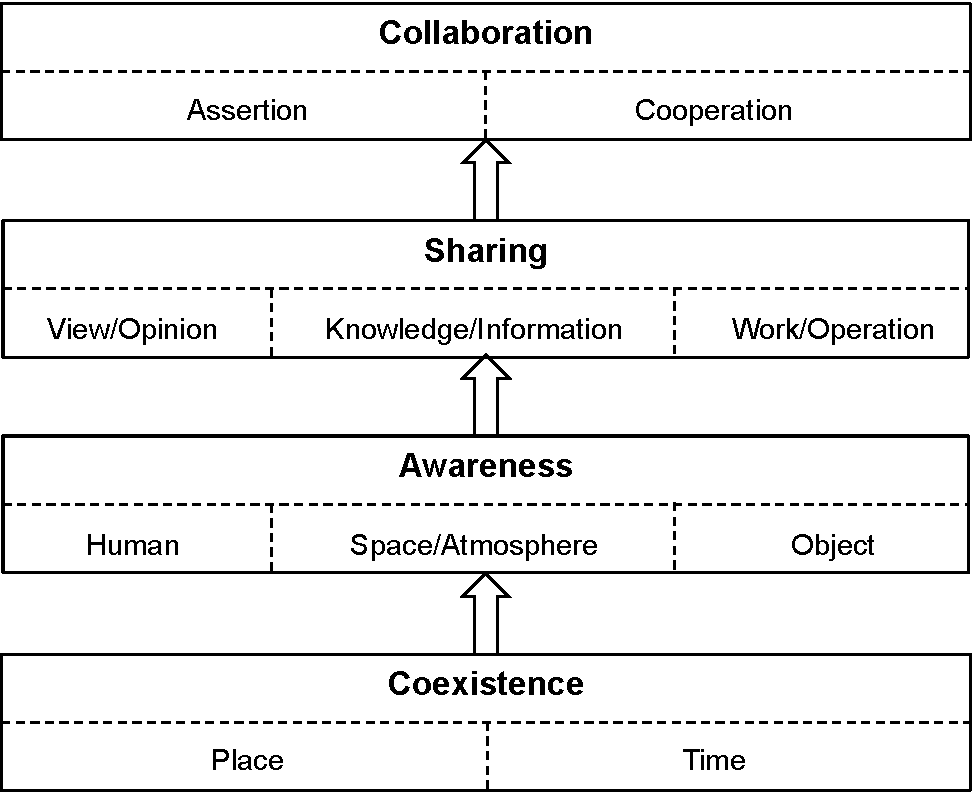
\includegraphics[width=0.6\textwidth]{figures/ch1/collab_model}
  \caption{\label{fig:1_collab_model}A hierarchical collaboration model from \citet{Okada2007Collab}.}
\end{figure}

\subsection{Groupware}
Being the central interest of CSCW, groupware is a type of computer-based systems designed to support a group of people to work together. \citet{Ellis1991Groupware} defined groupware as the following: ``computer-based systems that support groups of people engaged in a common task (or goal) and that provide an interface to a shared environment".

Groupware implementations can be grouped by a conceptual time-space matrix \citep{Johansen1988Groupware, Ellis1991Groupware} regardless of involved technology. As shown in Figure~\ref{fig:1_tsmatrix}, this matrix has a temporal dimension (whether users work the same time or asynchronously) and a spatial dimension (whether users are co-located or geographically distributed).

\begin{figure}[htb]
  \centering
  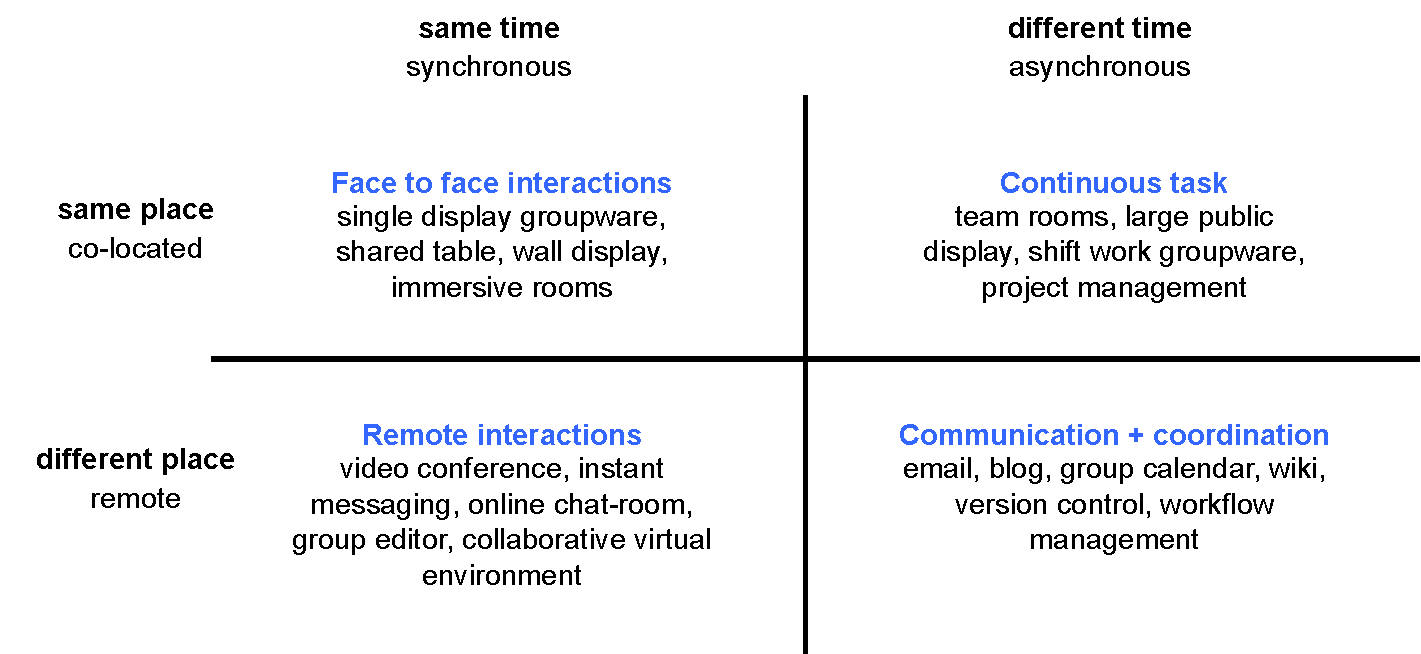
\includegraphics[width=\textwidth]{figures/ch1/tsmatrix}
  \caption{\label{fig:1_tsmatrix}The time-space matrix for groupware classification.}
\end{figure}

This typology of groupware based on time-space matrix is not aimed to provide strict rules to put every groupware application into one of the categories. Sometimes a given device can support both synchronous and asynchronous communications (e.g. two groups of users work on a wall display with results left by a previous group), and the used technology does not imply geographic distance between users (e.g. forwarding an email to a co-worker in the same room). However, it shows an overview of existing CSCW systems depending on the context of a system's use. It also offers a guideline for groupware design concerning temporal and spatial constrains. For example, synchronous applications need management of concurrent resource access and live communication between users, and groupware connecting remote users need to carefully choose the network architecture (server-client, peer-to-peer, etc.) to be used and to take into consideration the network latency.

Another taxonomy by \citep{Grudin2012Taxonomy} divides collaborative activities into three functional categories: communication, information sharing and coordination. The accomplishment of a collaborative task often requires all three types of activities. For example, when several authors of a book use a group editor to finish their work together, they need to have a shared version of the document and a clear assignment of different unfinished parts to corresponding authors, and also real-time communications by means of instant messages or audio meetings and asynchronous communications by leaving comments and annotations.


\subsection{Collaborative Virtual Environment}
\subsubsection{Definition}
A Collaborative Virtual Environment (CVE) refers to a virtual environment that enables multiple users to interact and to achieve collaborative tasks. CVEs provide a potentially infinite, graphically realized digital landscape within which multiple users can interact with each other and with simple or complex data representations \citep{Churchill1998CVE}. 

CVE differs from traditional groupware applications (e.g. email, instant messages, video conference, etc.) in that, instead of connecting people from different locations, CVEs create a virtual world and ``put" users and task related information directly in that world. This virtual world naturally provides users with a common spatial and social context for collaboration. CVEs are also different from other content sharing groupware such as group editors and group calendars because CVEs are multi-function and multi-purpose platforms that can support many forms of communication both for routinized and highly flexible tasks. Users have more degrees of control over the communication with others (free to navigate and encounter people) and more types of interactions with digital objects inside a malleable virtual space.

A lot of CVE applications exist from early prototypes (e.g. DIVE \citep{Carlsson1993DIVE}, NPSNET \citep{Macedonia1994NPSNET} etc.) appeared during 1990's (Figure~\ref{fig:1_cve:dive}), to more developed systems like MASSIVE-3 \citep{Greenhalgh2000MASSIVE} and ANTS \citep{Lopez2003ANTS}, etc. The general framework of CVE is gradually stabilized and standardized since then. Now mature CVE systems are widely applied and become the major trend in the game industry, there are enormous commercial products like online communities (e.g. Active Worlds\footnote{https://www.activeworlds.com}) (Figure~\ref{fig:1_cve:aw}) and collaborative games like MMORPGs\footnote{Massively Multiplayer Online Role-Playing Games} which attract millions of users \citep{Brown2004CSCW}. More information about the history and current status of CVEs are presented by \citet{Joslin2004CVE}.

\begin{figure}[htb]
  \begin{subfigure}{.5\textwidth}
    \centering
    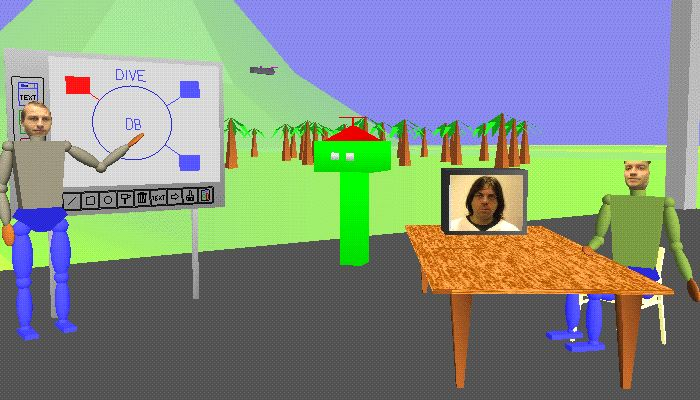
\includegraphics[width=\linewidth]{figures/ch1/dive}
    \caption{A virtual meeting within the DIVE platform.}
    \label{fig:1_cve:dive}
  \end{subfigure}
  \begin{subfigure}{.5\textwidth}
    \centering
    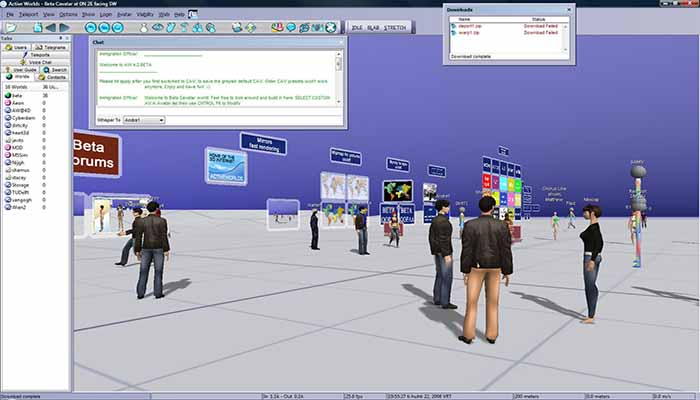
\includegraphics[width=\linewidth]{figures/ch1/activeworld}
    \caption{The Cavatar world from Active Worlds.}
    \label{fig:1_cve:aw}
  \end{subfigure}
  \caption{\label{fig:1_cve} Some examples of existing CVE applications.}
\end{figure}


\subsubsection{Issues and Challenges}
\label{sec:cve-issue}
The emergence of CVEs comes along with technical issues due to the complexity of such system. Supporting rich social interaction in densely populated virtual worlds requires addressing a variety of technical challenges. Here is a list of technical issues that need to be addressed inspired by the work of \citet{Benford2001CVE} and \citet{Joslin2004CVE}:

\begin{itemize}
\item Scene management: how to merge events and keep data consistency among different sites, how to segment a virtual world into smaller sections \citep{Kazman1993Making};
\item Network topology: choose among server-client, peer-to-peer or hybrid structure to reduce traffic loads and improve data distribution efficiency;
\item Compression: how to compress the data to be transmitted knowing that real time interaction between multiple users can generate huge amount of data, especially with sophisticated virtual human \citep{Capin1998Efficient};
\item Personal viewpoint: design software model to support ``subjective" view on the shared world \citep{Smith1996CVE};
\item Human computer interface: using virtual reality technology to convey more information for natural interaction and social communication;
\item etc.
\end{itemize}

Human factors are also crucial to the design and effective use of CVEs as a new type of social community. Here we group research questions around four topics: 

\begin{itemize}
\item Social conventions: are the social conventions in the real world still applicable in the shared virtual world \citep{Becker1998Social}? What has or has not changed?
\item User embodiment: how the virtual representations (simple object, robot, humanoid avatar, etc.) influence their communication? How to design the body image of a user to provide information such as identity, activity, availability, mood and many other factors \citep{Benford1995Embodiment}? 
\item Awareness: how to be aware of other people's intention and perceptual capabilities (e.g. size of field of view) in the virtual world \citep{Benford1994Awareness}?
\item Social communication: how social communications are supported in CVEs compared to cases in real world \citep{Bailenson2006Long}?
\end{itemize}

\citet{Otto2006Review} also give a similar summary of factors that influence collaboration in CVEs by grouping them into different levels:

\begin{itemize}
\item Application factors: task design, usability, performance, workflow ,etc.
\item Human factors: presence, social human communication, etc.
\item Technology factors: immersion, field of view (FoV), user interface, data distribution, etc.
\end{itemize}

\subsection{Summary}
This second part of Chapter \ref{chapter:context} summarizes characteristics of collaborative work in the real world and their implications for the design of computer supported collaboration systems (groupware). CVE as a flexible and multi-function platform attracts research interests from both CSCW and virtual reality communities. Although there are still many technical and human-related issues to be solved, CVEs already show great potential for supporting efficient and seamless collaboration in a rich social context.


% -------------------------------------------------------------------------------------------------

\section{Immersive Collaborative Virtual Environment}
As stated in the previous section, CVE is developing as a convergence of research interests within CSCW and VR communities. On the one hand, most existing virtual reality systems (e.g. CAVEs or HMD-based systems) can offer high level of multi-sensory immersion for a single user (except multi-user systems that we will talk about in Chapter \ref{chapter:colocated_colab}), so it is interesting to make connexions between these (remote) immersive systems by CVE technology to enable group immersion. On the other hand, with the progress of telecommunication technology and computer science (computer graphics, high performance computing, etc.) in recent years, many low-level issues of CVEs are already solved or we can say, are no longer the bottleneck for CVE usage. However, desktop-based CVEs with traditional human-computer interface have still limited support for social human communications compared to face-to-face interaction in the real world, and the lack of sensorial feedback makes it difficult for users to feel ``being in the virtual world" and impairs their task performance \citep{Narayan2005Quantifying, Nam2008Roles}, so it is important to introduce behavioral interfaces for CVEs to convey more social cues for human communication and to improve the immersion level.

As a consequence, more immersive CVEs are implemented with various hardware and software solutions. With the ``perception, decision and action" loop as shown in Figure~\ref{fig:1_loop}, we can apply this loop in a multi-user situation and extend it to illustrate the conceptual framework of immersive CVEs (Figure~\ref{fig:1_multi_loop}). In this shared virtual world, users' ``perception, decision and action" loops are interconnected as one user's action could affect other users' perception of the virtual world.

\begin{figure}[htb]
  \centering
  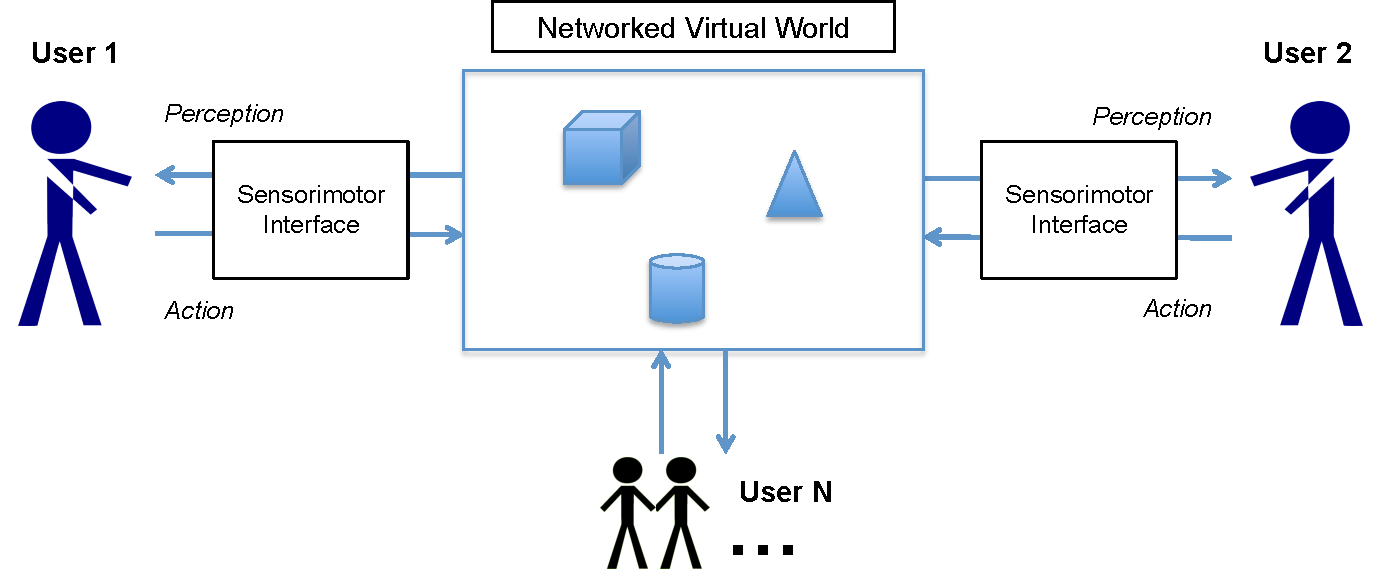
\includegraphics[width=0.9\textwidth]{figures/ch1/multi_loop}
  \caption{\label{fig:1_multi_loop}The conceptual framework of immersive CVE designed for the multi-user collaboration.}
\end{figure}

This new networked immersive experience not only changes the way people interact with objects in the virtual world, but also has impacts on how users communicate and interact with each other. The following part of this section will present in more details about different research questions and existing work around CVEs and immersive CVEs from a user-centered perspective.

\subsection{User Representation}
As discussed in section~\ref{sec:cve-issue}, users need virtual representations in the shared virtual space in order to be perceived by others. The virtual representation of users, or can be called user embodiment as explained by \citep{Benford1995Embodiment}, ``concerns the provision of users with appropriate body images so as to represent them to others (and also to themselves) in collaborative situations." Information conveyed by such representation could be position, identity, activity, availability and many other factors \citep{Thalmann2001VHR}. In an immersive virtual environment, this embodiment plays a crucial role for user interaction and communication \citep{Slater1994Body}, it is also helpful (sometimes indispensable) for users to get self-related information. For example, a user equipping an HMD perceives the virtual world from a first-person viewpoint, but the perception of his/her real body is completely blocked so a virtual body image can help to ``recreate the missing body" \citep{Lok2003Effects, Mohler2010Effect}. Moreover, according to the task that the users need to achieve in the virtual context, social representation of self may be provided through dedicated virtual clothings and/or virtual tools. 

The virtual representation of a user is usually a graphic entity, although sometimes a spatialized audio source is also sufficient for certain tasks. Three dimensional graphic recreations of human body (i.e. avatar) can be in extremely different forms, both in terms of morphology and photorealism (rendering style and Levels of Detail (LoD)) \citep{Garau2006Fidelity}. We can have from simple humanoid robots to highly detailed realistic virtual humans. For example, as shown by Figure~\ref{fig:1_vrep:rep_avatar_low}, users in MASSIVE-1 system are embodied in T-shaped robots with their names on top, they can easily get each other's information as position, orientation, identity and availability (avatars of off-line users are lying down) \citep{Greenhalgh1995MASSIVE}. Avatars as used by \citet{Roberts2004SSH} can convey more non-verbal information such as gestures and postures (Figure~\ref{fig:1_vrep:rep_avatar_high}). Users can also be represented by live video streams shown on 3D windows (billboards) \citep{Hayashi2007Immersive} (Figure~\ref{fig:1_vrep:billboard}). Another interesting method developed by \citet{Ogi2001SteAva} introduces an animated video avatar based on live video capture to avoid mesh-based avatar design. This 2.5 dimensional video avatar is captured by a set of cameras so the avatar can be seen from a certain range of directions (Figure~\ref{fig:1_vrep:video_avatar}).

\begin{figure}[htb]
  \begin{subfigure}{.5\textwidth}
    \centering
    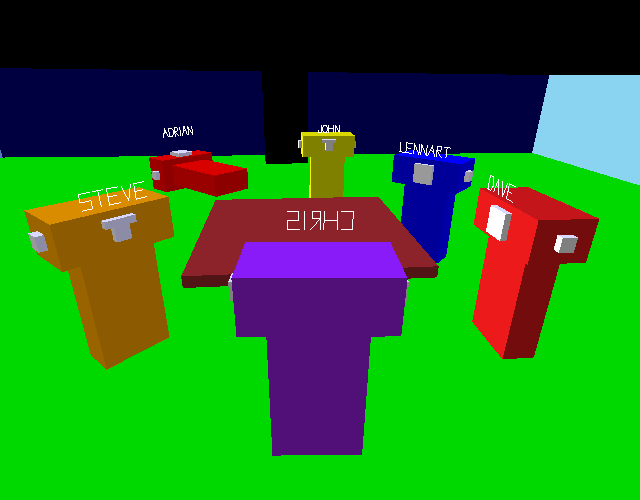
\includegraphics[width=0.9\linewidth]{figures/ch1/rep_avatar_low}
    \caption{Users represented by T-shaped robots in MASSIVE-1.}
    \label{fig:1_vrep:rep_avatar_low}
  \end{subfigure}
  \begin{subfigure}{.5\textwidth}
    \centering
    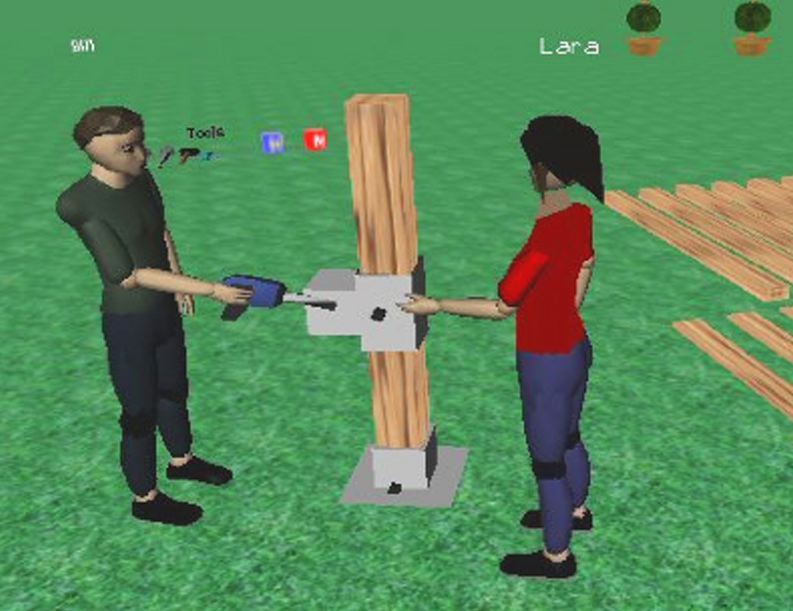
\includegraphics[width=0.9\linewidth]{figures/ch1/rep_avatar_high}
    \caption{Simple avatars with higher level of detail.}
    \label{fig:1_vrep:rep_avatar_high}
  \end{subfigure}
  \begin{subfigure}{.5\textwidth}
    \centering
    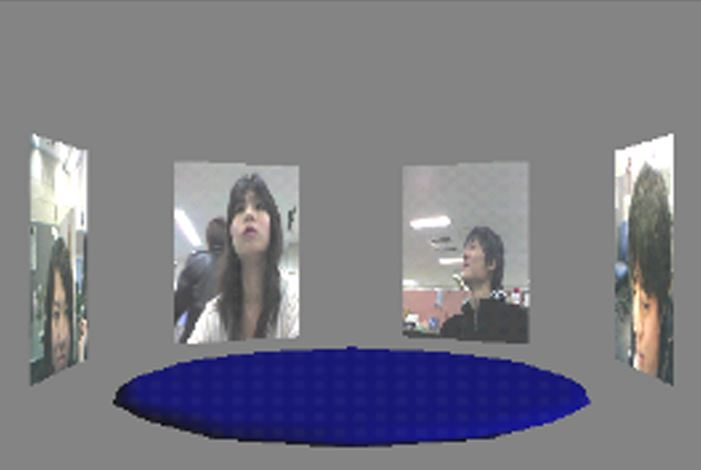
\includegraphics[width=0.9\linewidth]{figures/ch1/rep_billboard}
    \caption{Users having a round table meeting through a set of video streams shown on 3D billboard.}
    \label{fig:1_vrep:billboard}
  \end{subfigure}
  \begin{subfigure}{.5\textwidth}
    \centering
    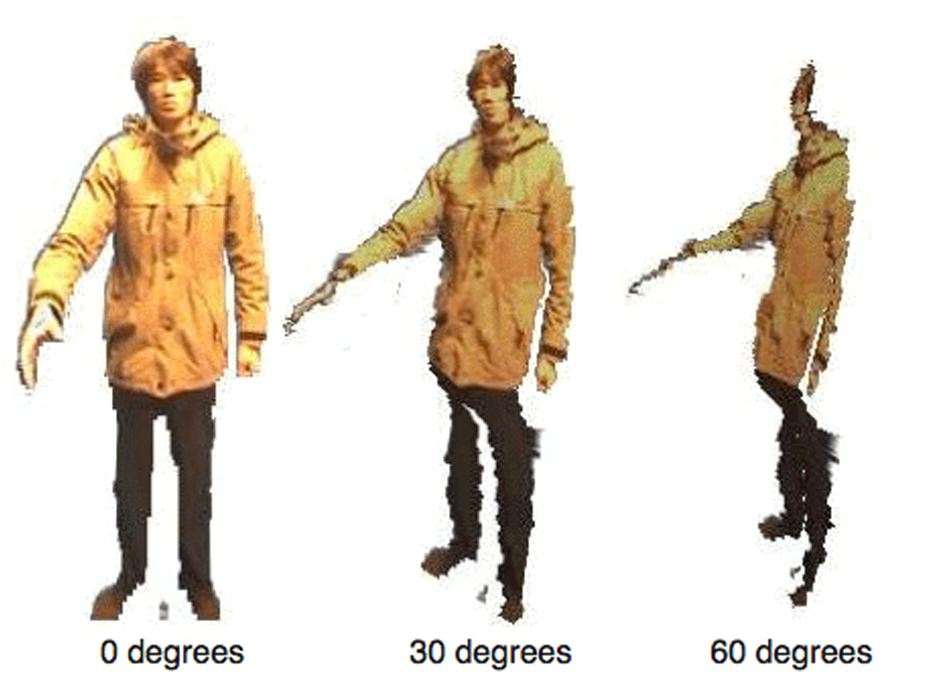
\includegraphics[width=0.9\linewidth]{figures/ch1/rep_video_avatar}
    \caption{Live video texture based 2.5 dimensional video avatar seen from various directions.}
    \label{fig:1_vrep:video_avatar}
  \end{subfigure}
  \caption{\label{fig:1_vrep} Some examples of user's virtual representation in CVEs.}
\end{figure}

In immersive CVEs (as well as desktop CVEs), high fidelity virtual humans are not always preferred against simple avatars. First, as human body is extremely complex which contains hundreds of muscles and joints, a virtual model replicating exactly the human body in real time is both challenging and costly in terms of computational and network resources. So generally we only need avatars that are ``good enough" for the given task depending on the trade-off between fidelity and efficiency. Second, the resemblance between the real user and his/her avatar is not always found to be beneficial due to the uncanny valley \citep{Mori1970Uncanny,Mori2012Uncanny}, which has led to lots of discussions and research works in the fields of robotics and computer animation. At last, as collaborative works are task-oriented, certain tasks proceeded in non-realistic virtual worlds (e.g. scientific data visualization, imaginary artistic world) do not necessarily require virtual humans. User representations are not limited to humanoid avatars and can be any kind of ``beings" or objects according to the context of the virtual world, sometimes realistic virtual humans can even be ``distractors" for the ongoing task.

Overall, a lot of technical issues still present regarding avatar modeling, animation and motion capture technology if we look for realistic virtual humans inside immersive CVEs. \citet{Magnenat2006Interactive} give a good review of research work on interactive virtual humans in real-time virtual environments.


\subsection{User Communication}
\label{sec:user-com}
Social human communication (SHC) contains four primary elements: verbal and non-verbal communication, references to objects and references to the environment \citep{Burgoon1994Human}. \citet{Bolt1980Put}'s ``put-that-there" command gives a good illustration of these four elements despite the fact that he was talking to a computer: he was speaking (verbal communication) while pointing (non-verbal communication) to an object (reference to objects) and ``there" refers to a certain place in the virtual environment. 

When working with CVEs, references to objects and environment can be easily understood as all users share the same objects and environment. Regarding verbal and non-verbal communications, while it is relatively easy to enable direct verbal communication (spatialized audio requires more complex setup) between users, it is complicated to convey non-verbal communications through network.

Recent research shows increasing importance of non-verbal communications during networked collaborative work \citep{Guye1999Nonverbal, Roberts2004SSH} including gestures \citep{Dodds2011Talk}, postures \citep{Normand2012Full}, eye contact \citep{Bailenson2002Gaze, Garau2003Impact} and facial expressions \citep{Boker2009Effects}. With desktop-based CVEs, we can play pre-recorded animations to carry out non-verbal communication as implemented in many multi-player games. However, this method is cumbersome and all personal information can not be conveyed. Immersive CVEs allow users connected by network to ``step into each other's world" and provide the closest resemblance of co-location compared to other tele-collaboration technologies \citep{Wolff2007Review}. In immersive CVEs, non-verbal cues such as gestures and postures, can be better supported by motion tracking technology combined with real time avatar animations.

Social scientists also start to use immersive CVEs as a tool to study human behavior in face-to-face communication by introducing biases in the virtual simulation. For example, \citet{Ennis2010Seeing} investigated human sensitivity to audio mismatches and visual desynchronization using motion capture data (Figure~\ref{fig:1_commu}). 

\begin{figure}[htb]
  \centering
  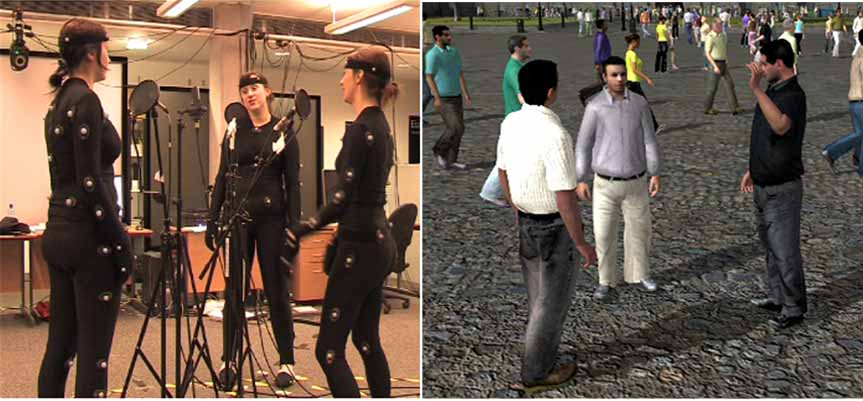
\includegraphics[width=0.9\textwidth]{figures/ch1/commu_study}
  \caption{\label{fig:1_commu} Avatars animated by motion capture data for behavioral study.}
\end{figure}

\subsection{User Interaction}
During closely-coupled collaboration, user interaction mainly concerns object co-manipulation among multiple users. Co-manipulation means that multiple users can act on the same object simultaneously, which belongs to level 3 cooperation according to the classification given by \citet{Margery1999Framework}. To achieve co-manipulation, the system needs to manage concurrent access to an object by combining inputs from multiple users which often involve multimodel instructions \citep{Martin2011Reconfigurable}. As we presented in section~\ref{sec:3D_inter}, the way that users perform actions in the virtual world can be similar or very different from how we interact in the real world, metaphors are often needed to enable efficient interactions.

Two general solutions exist to support object co-manipulation: we can allocate the control of different attributes to different users, i.e. to separate degrees of freedom \citep{Pinho2002Cooperative} (e.g. one moves the object while another person changes its color); if we need to modify the same attribute, for certain type of attributes (e.g. position, size, etc.) we can take the average value of all the inputs \citep{Ruddle2002Symmetric}, or we can use sophisticated metaphors for real time concurrent manipulation, such as the SkeweR \citep{Duval2006Skewer}, 3-Hand Manipulation Technique \citep{Aguerreche2009Three}, etc.

Various research work prove that visual immersion \citep{Schroeder2001NIS, Roberts2003Gazebo, Narayan2005Quantifying} and multi-sensory feedback (especially haptic feedback) \citep{Nam2008Roles, Oguz2010Haptic} tend to provide users with higher level of presence and improve their task performance on object co-manipulation based on comparisons between desktop CVEs and immersive (or partially immersive) CVEs. \citet{Slater2000Small} also find that immersion has an impact on the social relationship between group members: the person who uses immersive display tended to emerge as the leader among users connected to the same CVE by desktop interfaces.


\subsection{From Presence to Copresence}
Users in an immersive virtual environment can have the feeling of presence (``being there") while a group of users connected to the same immersive CVE can experience copresence (``being there together") \citep{Slater2000Small}. Copresence differs from \textit{social presence} as the latter is a much broader concept which refers to the individual's experience of being with another person (not limited to CVEs) \citep{Schroeder2002Copresence}.

Copresence itself can also have different implications and can be interpreted as mode of being with others, or as sense of being with others \citep{Zhao2003Taxonomy}. It is difficult to separate copresence in the sense of co-immersiveness from copresence in the sense of doing things together \citep{Schroeder2002Copresence} as the task duration and amount of interactions during collaboration seem to influence the feeling of being together with other people. Existing studies \citep{Slater2002Meeting, Garau2003Thesis} find a link between copresence and avatar fidelity in terms of appearance and behavior: even minimal behavioral cues can enhance the perceived quality of social interaction in VEs, however, the consistency between the fidelity of the avatar's behavior and its appearance is essential. \citet{Bailenson2005Copresence}'s experiment showed that copresence was lowest when there was a large mismatch between the appearance and behavioral realism of an embodied agent, though the ``uncanny valley" was not discussed due to the limited test conditions.

Several other concepts, such as mutual awareness, connected presence, engagement and virtual togetherness, have similar meaning with copresence. Detailed descriptions and discussions on these concepts can be found in \citet{Schroeder2006Being}'s review which facilitates understanding of group behavior in networked virtual environment. 


\subsection{Summary}
This last section presents different aspects of collaboration in CVEs from user-centered perspective: how users are presented and perceived in the virtual environment, how they communicate and interact to achieve a common goal. Being the combination of CVEs with virtual reality technology, immersive CVEs provide users with novel experience in terms of perception and interaction which makes a further step towards seamless collaboration among networked users. 


\section{Conclusion}
This chapter contextualizes the research by presenting an overview of relevant notions for collaboration in virtual environment, especially in immersive systems where users interact through behavioral interfaces. With technical progress of CVEs and VR interfaces, more immersive CVEs support user groups for collaborative work. Novel interaction paradigms are needed to ensure users' mutual awareness and to facilitate user communication and interaction, also to keep their level of immersion in the virtual environment. 

When multiple users are physically situated in the same immersive system for co-located collaboration, the coexistence of real and virtual information create a more complicated mixed context. The next chapter will concentrate on co-located collaboration in immersive virtual environment with the driving motivation, addressed issues, and the approach taken in this thesis.